\documentclass[tikz,border=10pt]{standalone}
\usetikzlibrary{shapes.geometric,backgrounds,calc}
\tikzset{
  basic box/.style = {
    shape = rectangle,
    align = center,
    draw  = #1,
    fill  = #1!25,
    minimum width = 2cm,
    minimum height = 0.8cm,
    rounded corners}
}
\begin{document}
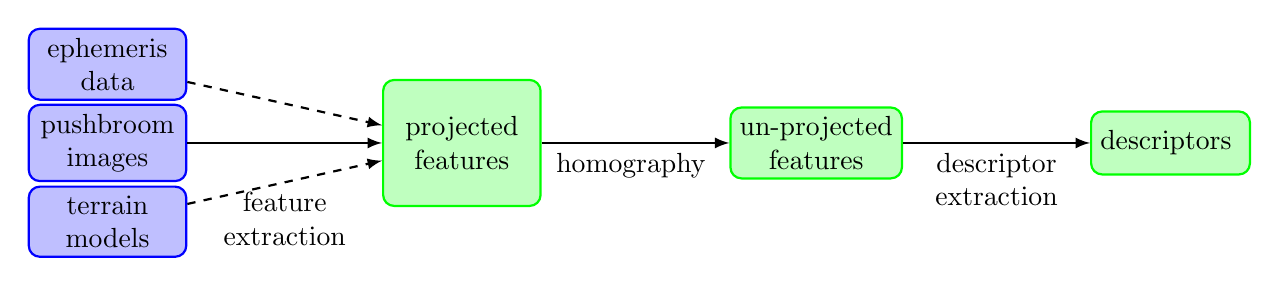
\begin{tikzpicture}[node distance = 4.5cm, thick, nodes = {align = center}, >=latex]
  \node[basic box = blue, anchor = west, yshift = -1cm] (terrain) { terrain \\ models };
  \node[basic box = blue, anchor = west, yshift = 1cm] (ephemeris) { ephemeris \\ data };
  \node[basic box = blue, anchor = west] (pbimagery) { pushbroom \\ images };
  \node[basic box = green, anchor = center, right of = pbimagery, minimum height = 1.6cm] (projfeatures) { projected \\ features };
  \node[basic box = green, anchor = west, right of = projfeatures] (features) { un-projected \\ features };
  \node[basic box = green, anchor = west, right of = features] (descriptors) { descriptors };
  \draw[->]    (pbimagery) -- (projfeatures);
  \draw[dashed,->]    (terrain) -- (projfeatures) node [midway,below] { feature \\ extraction };
  \draw[dashed,->]    (ephemeris) -- (projfeatures);
  \draw[->]    (projfeatures) -- (features) node [midway,below] { homography };
  \draw[->]    (features) -- (descriptors) node [midway,below] { descriptor \\ extraction };
\end{tikzpicture}
\end{document}
